%--------------------
% Packages
% -------------------
\documentclass[11pt,a4paper]{article}
\usepackage[utf8x]{inputenc}
\usepackage[T1]{fontenc}
%\usepackage{gentium}
\usepackage{mathptmx} % Use Times Font


\usepackage{comment}
\usepackage[pdftex]{graphicx} % Required for including pictures
\usepackage[pdftex,linkcolor=black,pdfborder={0 0 0}]{hyperref} % Format links for pdf
\usepackage{calc} % To reset the counter in the document after title page
\usepackage{enumitem} % Includes lists

\frenchspacing % No double spacing between sentences
\linespread{1.2} % Set linespace
\usepackage[a4paper, lmargin=0.1666\paperwidth, rmargin=0.1666\paperwidth, tmargin=0.1111\paperheight, bmargin=0.1111\paperheight]{geometry} %margins
%\usepackage{parskip}

\usepackage[all]{nowidow} % Tries to remove widows
\usepackage[protrusion=true,expansion=true]{microtype} % Improves typography, load after fontpackage is selected

\usepackage{lipsum} % Used for inserting dummy 'Lorem ipsum' text into the template

\usepackage[export]{adjustbox}
\usepackage{plantuml}
\usepackage{float}
\usepackage{indentfirst}
\usepackage{subcaption}

\usepackage{graphicx}

%\usepackage{etoolbox} % Adds '\clearpage' to every '\section command' (newpage).
%\pretocmd{\section}{\clearpage}{}{} 

\newcommand{\inputdiagram}[1]{\input{Diagrams/out/#1}}
\newcommand{\textwidthdiagram}[2][1]{%
  \resizebox{#1\textwidth}{!}{\inputdiagram{#2}}%
}

%-----------------------
% Set pdf information and add title, fill in the fields
%-----------------------
\hypersetup{ 	
pdfsubject = {Program Systems Engineering},
pdftitle = {itssoover},
pdfauthor = {Ignas Časas, Mykolas Marius Budrys, Augustas Kniška}
}

%-----------------------
% Begin document
%-----------------------
\begin{document} %All text i dokumentet hamnar mellan dessa taggar, allt ovanför är formatering av dokumentet

\begin{titlepage}
    \centering
    % Remove page numbering from title
    \thispagestyle{empty}
    
    % University name
    {\Large VILNIAUS UNIVERSITETAS\\
    Matematikos ir informatikos fakultetas}\par
    
    \vspace{3cm} % vertical space
    
    % Title of the work
    {\Large 2\textsuperscript{nd} Laboratory Work}\par
    \vspace{0.5cm}
    {\Large \textbf{itssoover}}\par
    {\Large \textbf{Design and Implementation}}\par
    
    \vspace{3cm}
    
    % Authors
    {\large
    Ignas Časas\\
    Mykolas Marius Budrys\\
    Augustas Kniška
    }\par
    
    \vspace{8cm}
    
    % Bottom of the page
    {\large
    Matematikos ir informatikos fakultetas\\
    Vilniaus universitetas\\
    Lietuva
    }\par
    
    \vfill

    \large 2025
    
\end{titlepage}

\tableofcontents
\newpage

\section{Context}
Our web-based application offers a variety of cognitive games. They are designed to improve cognitive skills like memory, attention, reaction time and math problem-solving skills. The platform is designed to be  accessible from anywhere with only a browser, no additional software is needed. Platform's games have different difficulties, users are able to choose the game's complexity based on their preference. Registered users have the luxury of tracking their own progress throughout the lifespan of their account. The games are designed to be engaging; however, the priority is to measure and boost cognitive improvement rather than just entertainment.

\subsection{Technology Stack}
\begin{itemize}
    \item \textbf{Frontend:} Built with Blazor for interactive C\#-based UI.
    \item \textbf{Backend:} .NET (C\#) Web API for business logic, user authentication, and statistics tracking.
    \item \textbf{Database:} SQLite for lightweight storage of user data and game progress.
\end{itemize}

\subsection{Content \& Accessibility Boundaries}
\begin{itemize}
    \item Games focus on cognitive improvement, not entertainment or storytelling.
    \item No complex mechanics (e.g., multiplayer or 3D).
    \item Web-based only—no mobile apps, downloads, or third-party integrations.
\end{itemize}

\subsection{Functionality \& Monetization}
\begin{itemize}
    \item Single-player only; no social features.
    \item No in-game purchases or microtransactions.
\end{itemize}



\section{Logical View}


\subsection{Class Diagram}

\begin{figure}[H]
     \centering
     \begin{adjustbox}{width=0.92\paperwidth,center}        \inputdiagram{class_diagram.tex}
     \end{adjustbox}
     \caption{Class Diagram}
     \label{fig:class_diagram}
\end{figure}

Figure~\ref{fig:class_diagram} illustrates the real class structure of the repository. Each class is a representation of an actual class in the project. The code-base is separated into three parts: client, server, and shared components. Not all architecture details are depicted in the diagram, but major elements are shown that illustrate the main underlying implementation. 


Client-side page components inherit from BlazerComponentBase. AccountPage and StatisticsPage are for tracking cognitive progress, SettingsPage is for the user's privacy settings. MathGamePage, SudokuGamePage, PairMatchingGamePage, and AimTrainerPage are for game-specific functionality. TimerService is used by each game to track time. All the pages are located in the "Client/Pages" folder, while TimeService is in the "Client/Services".


Server-side has three main parts. First, are the controllers like AccountScoreController, MathGameController, etc. They help to handle the incoming requests from the user side. Controllers are saved in the "Server/Controllers" folder. Second are the services like MathGameService, SudokuService, AimTrainerService, PairUpService, AccountScoreService and UserService. They handle the backend logic. Services are located in the "Server/Services" folder. Lastly, the Repositories like ScoreRepository and UserRepository. They handle the interactions with the database. Repositories are located in the "Server/Repositories" folder.


The shared resources mainly help by providing data models so that the server side and client side could easily interact. From the client class diagram, these would be the UserScoreDto<T> and AverageScoreDtomodels. They are located in the "Shared/Models" folder.

\subsection{Client States}

The relation between the components shown in the state diagrams and classes is explained in the Component section of the document.

\begin{figure}[H]
    \centering
    \begin{minipage}[b]{0.59\textwidth}
        \centering
        \textwidthdiagram{score_fetching_state.tex}
        \caption{AimTrainerPage Score Fetching}
        \label{fig:score_fetching_state}
    \end{minipage}
    \hfil
    \begin{minipage}[b]{0.4\textwidth}
        \centering
        \textwidthdiagram{user_authentication_state.tex}
        \caption{AccountAuthStateProvider State}
        \label{fig:user_authentication_state}
    \end{minipage}
\end{figure}

Figure~\ref{fig:score_fetching_state} outlines the asynchronous score
retrieval process by the AimTrainerPage component. Other Page components in
the Game Pages subsystem manage state in the same way. The state enters in
a "Loading Scores" state where a background call (GetUserHighScoreAsync())
fetches data. Depending on the outcome, the state branches into one of three
paths: it moves to "No Scores Found" if no score is returned, "Encountered
Error" if an error occurs, or "Showing Scores" if the scores are successfully
loaded. The User is shown different UI elements based on the AimTrainerPage
state. This structure ensures that the application handles different scenarios
gracefully while providing clear feedback to the user.

The AccountAuthStateProvider State diagram presented in
Figure~\ref{fig:user_authentication_state} defines the different possible
states of user authentication kept by AccountAuthStateProvider. The
component begins in an "Unauthenticated" state. When an external call
to mark the user as authenticated is made the component changes it's
internal state to "Authenticated". If a MarkUserAsLoggedOut call is made
and the AccountAuthStateProvider is in the "Authenticated" state the
method then reverts the component back to the "Unauthenticated" state. The
AccountAuthStateProvider component is user by the AccoutPage component. This
model clearly delineates the transitions between being logged in and logged
out, ensuring that the system maintains a secure and predictable user session
management process.

\subsection{Game States}

These state diagrams are made to represent the internal state kept by
the components of the GamePage when the game is being played.

\begin{figure}[H]
    \centering
    \begin{minipage}[b]{0.48\textwidth}
        \centering
        \textwidthdiagram{math_state.tex}
        \caption{MathGamePage State Representation}
        \label{fig:math_state}
    \end{minipage}
    \hfil
    \begin{minipage}[b]{0.48\textwidth}
        \centering
        \textwidthdiagram{aim_trainer_state.tex}
        \caption{AimTrainerPage State Representation}
        \label{fig:aim_trainer_state}
    \end{minipage}
\end{figure}

In Figure~\ref{fig:aim_trainer_state} we model our \textit{Aim Training} game. The
game starts by displaying a target, and upon the user's click, it transitions
to a state where the input is processed. If there is remaining time (i.e.,
[time\_left>0]), a new target is generated, looping back to the display state;
otherwise, the game ends. The \textit{ProcessingInput} state handles updating both
the failure count (if the target was missed) and the score.

Figure~\ref{fig:math_state} represents our arithmetic based \textit{Math Game}. It
begins by displaying an equation to the user. When an answer is submitted, the
system transitions to a validation state. The validation state is responsible
for both making an asynchronous call to the back-end for answer validation
and increasing the kept score if the answer was valid. If time remains,
a new question is generated and the process repeats; if not, the game
terminates. Modeling our game in this way highlights the cyclic gameplay
loop that emphasizes both continuous engagement and time-bound gameplay,
ensuring the game session concludes when the allotted time is exhausted.

\begin{figure}[H]
    \centering
    \begin{minipage}[b]{0.48\textwidth}
        \centering
        \textwidthdiagram{sudoku_state.tex}
        \caption{SudokuPage State Representation}
        \label{fig:sudoku_state}
    \end{minipage}
    \hfil
    \begin{minipage}[b]{0.48\textwidth}
        \centering
        \textwidthdiagram{pair_up_state.tex}
        \caption{PairUpPage State Representation}
        \label{fig:pair_up_state}
    \end{minipage}
\end{figure}

Figure~\ref{fig:sudoku_state} (The \textit{Sudoku} state diagram) captures
the interactive elements of playing our \textit{Sudoku} game. Initially, the board
is idle, waiting for user interaction. When a cell is selected, the state
changes, allowing the user to either deselect the cell, select another
cell, input a value, or submit the board for validation. Upon submission,
the system checks the board (by an asynchronous call to our API): if the
board is invalid, it redraws and returns to the idle state; if the board
is valid, the game ends. These states capture the essential user interactions
and decision points necessary for the logic puzzle.

The \textit{Pair Up} diagram (Figure~\ref{fig:pair_up_state}) details the
states of our memory-based matching game. The game starts with all cards being
shown to the user. The user selects his first card (which the user cannot
unselect), then his second card, prompting the system to evaluate whether the
selected pair matches. If there are still unpaired cards remaining, the game cycles
back to display the cards; if all pairs are successfully matched,
the game ends. This design effectively captures the iterative nature of this
game while clearly defining the conditions for continuation and termination.


\subsection{Information Model}

\begin{figure}[H]
    \centering
    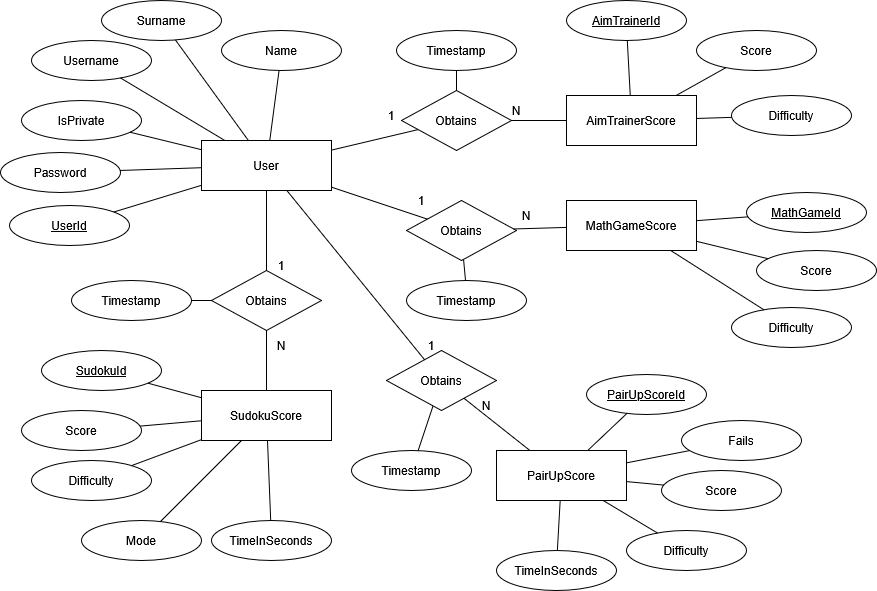
\includegraphics[width=\textwidth]{Diagrams/out/PNG/ER_Diagram_fix.drawio.png}
    \caption{ER Diagram}
    \label{fig:ER_diagram}
\end{figure}

In Figure~\ref{fig:ER_diagram}, the database structure of the system is displayed using an Entity-Relationship (ER) diagram. The diagram represents the entities (tables), their attributes, and the relationships between them. The database consists of five tables, each representing a key component of the system: User, AimTrainerScore, MathGameScore, PairUpScore, SudokuScore. Each score table has a direct relationship with the User table. Since a user can play multiple games and record multiple scores, the relationships are one-to-many. The Timestamp attribute is recorded directly within each score table.


\section{Development View}

\subsection{Package Diagram}

\begin{figure}[H]
    \centering
    \textwidthdiagram{Package_Diagram.latex}
    \caption{Package Diagram} 
    \label{fig:united_package}
\end{figure}

Figure~\ref{fig:united_package} provides an overview of how the codebase organization. For clarity and less abstraction, this diagram has some parts of the system that were not mentioned in the class diagram, such as "Shared/Enums", "Client/Components", and "Server/Database". This decision was made in order to simplify the class diagram while maintaining the key logical elements, but for the deployment diagram purposes they were added to provide more detail.

Similarly, as in the class diagram, the package diagram is split into Shared, Server, and Client folders. Not all folders are listed in the diagram, but the most important ones are. This was done to reduce clutter and make it easier to understand visually.

The Shared package highlights common elements across the project, such as data models and enumerations. A lot of parts in the client and server use these folders.

The server has controllers that await the client side requests, the controllers interact with services to perform certain tasks, such as saving a game record into the database. In this case, services will access the repositories' folder, which in turn will save a record in the database.

The Client has pages, components, and services. Pages interact with components and services, services send the requests to the server controllers.

The arrows indicate dependencies and illustrate how functionality is physically imported from one package to another.

\subsection{Component Diagrams}

\begin{figure}[H]
    \centering
    \textwidthdiagram{server_component_diagram.latex}
    \caption{Server Component Diagram}
    \label{fig:server_component_diagram}
\end{figure}

Figure~\ref{fig:server_component_diagram} illustrates the architecture of components from the Server package. Controllers provide API endpoints for frontend services, with each controller communicating with its corresponding service layer through well-defined interfaces. Services encapsulate the core business logic including game mechanics, user tracking, and account management. These services interact with other necessary services or repositories as needed. Data access is handled through repositories that abstract database operations.


The following outlines the mapping between components from a server component diagram and corresponding classes in a class diagram, organized by their respective subsystems or folders:
\begin{enumerate}[label=\textbf{\arabic*.}, ref=\arabic*]
    \item \textbf{Services}
        \begin{enumerate}[label=\textbf{\alph*.}, ref=\theenumi.\alph*]
            \item \textbf{User Services Subsystem}
                \begin{itemize}
                    \item \textbf{Component:} \texttt{UserTrackingService}
                        \begin{itemize}
                            \item \textbf{Equivalent Class:} \texttt{UserTrackingService}
                        \end{itemize}
                    \item \textbf{Component:} \texttt{UserService}
                        \begin{itemize}
                            \item \textbf{Equivalent Class:} \texttt{UserServices}
                        \end{itemize}
                    \item \textbf{Component:} \texttt{AccountScoreService}
                        \begin{itemize}
                            \item \textbf{Equivalent Class:} \texttt{accountScoreService}
                        \end{itemize}
                \end{itemize}
            \item \textbf{Game Services Subsystem}
                \begin{itemize}
                    \item \textbf{Component:} \texttt{AimTrainerService}
                        \begin{itemize}
                            \item \textbf{Equivalent Class:} \texttt{AimTrainerService}
                        \end{itemize}
                    \item \textbf{Component:} \texttt{SudokuService}
                        \begin{itemize}
                            \item \textbf{Equivalent Class:} \texttt{SudokuService}
                        \end{itemize}
                    \item \textbf{Component:} \texttt{PairUpService}
                        \begin{itemize}
                            \item \textbf{Equivalent Class:} \texttt{PairUpService}
                        \end{itemize}
                \end{itemize}
            \item \textbf{Math Game Services Subsystem}
                \begin{itemize}
                    \item \textbf{Component:} \texttt{MathGameServices}
                        \begin{itemize}
                            \item \textbf{Equivalent Class:} \texttt{MathGameService}
                        \end{itemize}
                    \item \textbf{Component:} \texttt{MathGenerationService}
                        \begin{itemize}
                            \item \textbf{Equivalent Class:} (Not in Class Diagram)
                        \end{itemize}
                    \item \textbf{Component:} \texttt{MathCalculationService}
                        \begin{itemize}
                            \item \textbf{Equivalent Class:} (Not in Class Diagram)
                        \end{itemize}
                    \item \textbf{Component:} \texttt{MathGameScoreboardService}
                        \begin{itemize}
                            \item \textbf{Equivalent Class:} (Not in Class Diagram)
                        \end{itemize}
                \end{itemize}
        \end{enumerate}
    \item \textbf{Controllers}
        \begin{enumerate}[label=\textbf{\alph*.}, ref=\theenumi.\alph*]
            \item \textbf{User Controllers Subsystem}
                \begin{itemize}
                    \item \textbf{Component:} \texttt{UserController}
                        \begin{itemize}
                            \item \textbf{Equivalent Class:} \texttt{UserController}
                        \end{itemize}
                    \item \textbf{Component:} \texttt{AccountScoreController}
                        \begin{itemize}
                            \item \textbf{Equivalent Class:} \texttt{AccountScoreController}
                        \end{itemize}
                \end{itemize}
            \item \textbf{Game Controllers Subsystem}
                \begin{itemize}
                    \item \textbf{Component:} \texttt{AimTrainerController}
                        \begin{itemize}
                            \item \textbf{Equivalent Class:} \texttt{AimTrainerController}
                        \end{itemize}
                    \item \textbf{Component:} \texttt{SudokuController}
                        \begin{itemize}
                            \item \textbf{Equivalent Class:} \texttt{SudokuController}
                        \end{itemize}
                    \item \textbf{Component:} \texttt{PairUpController}
                        \begin{itemize}
                            \item \textbf{Equivalent Class:} \texttt{PairUpController}
                        \end{itemize}
                    \item \textbf{Component:} \texttt{MathGameController}
                        \begin{itemize}
                            \item \textbf{Equivalent Class:} \texttt{MathGameController}
                        \end{itemize}
                \end{itemize}
        \end{enumerate}
    \item \textbf{Repositories Folder}
        \begin{itemize}
            \item \textbf{Component:} \texttt{User Repository}
                \begin{itemize}
                    \item \textbf{Equivalent Class:} \texttt{UserRepository}
                \end{itemize}
            \item \textbf{Component:} \texttt{Score Repository}
                \begin{itemize}
                    \item \textbf{Equivalent Class:} \texttt{ScoreRepository}
                \end{itemize}
        \end{itemize}
    \item \textbf{Database Folder}
        \begin{itemize}
            \item \textbf{Component:} \texttt{UserDbContext}
                \begin{itemize}
                    \item \textbf{Equivalent Class:} (Not in Class Diagram)
                \end{itemize}
        \end{itemize}
\end{enumerate}

\begin{figure}[H]
    \centering
     \begin{adjustbox}{width=0.92\paperwidth,center}
         \inputdiagram{client_components.tex}
     \end{adjustbox}
    \caption{Client Package Component Diagram}
    \label{fig:client_components}
\end{figure}

Figure~\ref{fig:client_components} visualizes the components inside the Client package.  The pages
are divided into two subsytems: User Pages - for handling client-side
authentication and account managment related views, Game Pages - for pages
containing game implementations. The Page components interface with components
from both the Account Services and Game Services subsystems.  The service
components are responsible for storing game or account related data locally,
substituting parts of game logic implementation or making HTTP requests to
the Web API. Hence they require HTTP API Endpoints for their functionality.

The following outlines the mapping between components from a client component diagram and corresponding classes in a class diagram:
\begin{enumerate}[label=\textbf{\arabic*.}, ref=\arabic*]
    \item \textbf{Services}
        \begin{enumerate}[label=\textbf{\alph*.}, ref=\theenumi.\alph*]
            \item \textbf{Timer Service}
                \begin{itemize}
                    \item \textbf{Component:} \texttt{TimerService}
                        \begin{itemize}
                            \item \textbf{Equivalent Class:} \texttt{TimerService}
                        \end{itemize}
                \end{itemize}
            \item \textbf{Account Services Subsystem}
                \begin{itemize}
                    \item \textbf{Component:} \texttt{AccountScoreService}
                        \begin{itemize}
                            \item \textbf{Equivalent Class:} \texttt{AccountScoreService}
                        \end{itemize}
                    \item \textbf{Component:} \texttt{AccountService}
                        \begin{itemize}
                            \item \textbf{Equivalent Class:} (Not in Class Diagram)
                        \end{itemize}
                    \item \textbf{Component:} \texttt{AccountAuthStateProvider}
                        \begin{itemize}
                            \item \textbf{Equivalent Class:} (Not in Class Diagram)
                        \end{itemize}
                \end{itemize}
            \item \textbf{Game Services Subsystem}
                \begin{itemize}
                    \item \textbf{Component:} \texttt{SudokuService}
                        \begin{itemize}
                            \item \textbf{Equivalent Class:} \texttt{SudokuService}
                        \end{itemize}
                    \item \textbf{Component:} \texttt{MathGameService}
                        \begin{itemize}
                            \item \textbf{Equivalent Class:} \texttt{MathGameService}
                        \end{itemize}
                    \item \textbf{Component:} \texttt{PairUpService}
                        \begin{itemize}
                            \item \textbf{Equivalent Class:} \texttt{PairUpService}
                        \end{itemize}
                    \item \textbf{Component:} \texttt{AimTrainerService}
                        \begin{itemize}
                            \item \textbf{Equivalent Class:} \texttt{AimTrainerService}
                        \end{itemize}
                \end{itemize}
        \end{enumerate}
    \item \textbf{Pages}
        \begin{enumerate}[label=\textbf{\alph*.}, ref=\theenumi.\alph*]
            \item \textbf{User Pages Subsystem}
                \begin{itemize}
                    \item \textbf{Component:} \texttt{ScorePage}
                        \begin{itemize}
                            \item \textbf{Equivalent Class:} \texttt{StatisticsPage}
                        \end{itemize}
                    \item \textbf{Component:} \texttt{AccountPage}
                        \begin{itemize}
                            \item \textbf{Equivalent Class:} \texttt{AccountPage}
                        \end{itemize}
                    \item \textbf{Component:} \texttt{SettingsPage}
                        \begin{itemize}
                            \item \textbf{Equivalent Class:} \texttt{SettingsPage}
                        \end{itemize}
                \end{itemize}
            \item \textbf{Game Pages Subsystem}
                \begin{itemize}
                    \item \textbf{Component:} \texttt{AimTrainerPage}
                        \begin{itemize}
                            \item \textbf{Equivalent Class:} \texttt{AimTrainerPage}
                        \end{itemize}
                    \item \textbf{Component:} \texttt{SudokuPage}
                        \begin{itemize}
                            \item \textbf{Equivalent Class:} \texttt{SudokuPage}
                        \end{itemize}
                    \item \textbf{Component:} \texttt{MathGamePage}
                        \begin{itemize}
                            \item \textbf{Equivalent Class:} \texttt{MathGamePage}
                        \end{itemize}
                    \item \textbf{Component:} \texttt{PairUpPage}
                        \begin{itemize}
                            \item \textbf{Equivalent Class:} \texttt{PairMatchingGamePage}
                        \end{itemize}
                \end{itemize}
        \end{enumerate}
\end{enumerate}

\section{Process View}

\subsection{Sequence Diagrams}

\begin{figure}[H]
    \centering
     \begin{adjustbox}{width=0.92\paperwidth,center}
         \inputdiagram{aim_trainer_page_sequence.tex}
     \end{adjustbox}
     \caption{\textit{Aim Trainer} Page Loading Sequence}
    \label{fig:aim_trainer_page_sequence}
\end{figure}
In order to visualize the way in which score fetching works for all of
our games we will do a case analysis on the \textit{AimTrainerPage} component.
Figure~\ref{fig:aim_trainer_page_sequence} illustrates the process flow
when a player opens the Aim Trainer page. Initially, the page immediately
requests the username from the authentication provider component. After
this, an initial page is shown to the user with an icon to indicate the fact
that scores are being loaded. Once the username is retrieved and confirmed
not to be null, the page initiates an asynchronous call to the client-side
service to fetch the player's high score. The client service makes an HTTP GET
request to an endpoint provided by the Aim Trainer controller, which, in turn,
invokes the server-side service. The server service interacts with the Score
Repository and User Database Context to locate the corresponding user and
their scores. Depending on whether the user and score exist, the repository
returns either a list of scores or an empty list. The server service then
filters the result to extract the highest score, and this filtered result
is passed back up the chain and sent back as JSON (if a score was found)
and an empty response otherwise. After parsing and unwrapping the data on
the client side, the Aim Trainer page updates its display, showing either the
retrieved high score or a "Not Found" message if no score was found. Finally,
the updated view is presented to the player. This is the way all of our
games implement the score fetching functionality.

\begin{figure}[H]
    \centering
     \begin{adjustbox}{width=0.92\paperwidth,center}
        \inputdiagram{aim_trainer_set_score_sequence.tex}
     \end{adjustbox}
    \caption{Aim Trainer Score Setting Sequence}
    \label{fig:aim_trainer_set_score_sequence}
\end{figure}

This sequence diagram (Figure~\ref{fig:aim_trainer_set_score_sequence})
is an example of the process initiated by finishing a play session in one
our games \textbf{WHILE AUTHENTICATED} (otherwise no such process occurs
on the client side). Once again we analyze only the AimTrainerPage, however
other pages operate in a similar way. Once the game ends, the page calls the
client-side service to save the player's score asynchronously. The client
service wraps the score within a DTO and forwards it via an HTTP POST request
to an API endpoint provided by the Aim Trainer controller. The controller
then uses the server-side service component to process the request. The
server-side service unwraps the DTO and uses an interface provided by the
Score Repository, which attempts to find the corresponding user within the
given database context.  If the user is found, the repository attempts to
add the score to the database; if an exception occurs during this process it
is caught by the controller and the controller decides the appropriate HTTP
error code to return (HTTP 500 for DB exceptions, or HTTP 400 when a user
is not found, indicating that a deceptive request might have been sent). If
the user is found, and the insertion process is successful the controller
returns a HTTP 200 OK code. Finally, the result is propagated back through
the client service to the Aim Trainer page, updating the UI accordingly.

\subsection{Activity Diagram}
\begin{figure}[H]
    \centering
     \begin{adjustbox}{width=0.92\paperwidth,center}
        \inputdiagram{leaderboard_activity.tex}
     \end{adjustbox}
    \caption{Leaderboard Loading Diagram}
    \label{fig:leaderboard_activity}
\end{figure}

To show the way in which leaderboard scores get loaded by the components in
the Game Pages subsystem we show an example of how the PairUpPage component
executes this functionality (Fig.~\ref{fig:leaderboard_activity}.  This process
is initiated by a Player navigating to the Pair Up game page. The PairUpPage
component then handles showing the Player the needed loading icons and making
an asynchronous call chain to fetch the leaderboards from the API in parallel.
The HTTP request is sent by the PairUpService(C) (C - indicating the client
side service) component.  The PairUpController component handles receiving
the request and passing it along to the PairUpService(S) (S - indicating
the server side service).  PairUpService(S) then receives the leaderboard
entries by using the ScoreRepository component and filters out the entries
of players which have chosen to hide their high scores.  It then returns the
entries to the controller which sends a response to the initial HTTP request.
The PairUpService(C) parses the response and throws an exception if it did
not receive a valid response.  The PairUpPage component then handles logic
for updating the final page view.

\section{Physical View}
\subsection{Deployment}
\begin{figure}[H]
    \centering
    \begin{adjustbox}{width=0.92\paperwidth,center}
        \inputdiagram{deployment_diagram.tex}
     \end{adjustbox}
    \caption{Deployment Diagram}
    \label{fig:deployment_diagram}
\end{figure}

Figure~\ref{fig:deployment_diagram} illustrates the deployment of the web
application, which consists of a client-side Blazor WebAssembly (WASM)
front-end app accessed from a browser and a back-end Web API hosted on
an Azure server. The client browser runs the provided .NET WASM runtime,
running Client.dll as an executable. The backend operates in a Linux (Ubuntu)
environment within Azure, where the .NET runtime hosts the Server.dll
executable. The Server.dll contains an entry point for the Web API, the
Client.dll contains an entry point for the Blazor App. Data is persisted using
an SQLite database (SQLite is built into the Server.dll). Communication
between the client and server occurs over HTTPS, ensuring secure data
transmission. This design enables a lightweight client while leveraging
cloud infrastructure for back-end processing and storage of user and game data.

\subsection{CI/CD}

\begin{figure}[H]
        \centering
        \textwidthdiagram[0.8]{CI.tex}
        \caption{CI Pipeline}
        \label{fig:CI_pipeline}
\end{figure}
Figure~\ref{fig:CI_pipeline} focuses on our pull request (PR) validation
workflow. Triggered by any pull request targeting the main branch, this
pipeline starts by setting up a linux environment (latest Ubuntu) and
executing a series of steps: checking out the code, setting up the .NET
environment, restoring dependencies, building the solution, and running
tests. The critical decision point here assesses whether all tests pass. If
they do, the PR status is marked as passing, signaling readiness for review
and potential merge. If any tests fail, the pipeline marks the PR as failing
and prevents it from being merged, thus upholding code quality and integrity
before changes are integrated into the main branch.

\begin{figure}[H]
    \centering
    \textwidthdiagram[0.8]{CD.tex}
    \caption{CD Pipeline}
    \label{fig:CD_pipeline}
\end{figure}
Figure~\ref{fig:CD_pipeline} illustrates our CD pipeline using GitHub
Actions. The whole process is excecuted on a linux(latest Ubuntu)
environment. The process begins when a push to the main branch or a manual
trigger starts the pipeline. Within the "Build and Test Job" partition,
the pipeline checks out the repository, sets up the .NET environment,
restores dependencies, and builds the application. After running tests,
the workflow evaluates the outcome: if the tests succeed, it proceeds to
publish the application and upload the resulting artifact; if any test fails,
the deployment is aborted immediately. Following a successful build and test
phase, the "Deploy Job" partition retrieves the artifact from the previous
step and deploys it to Azure, ensuring that only verified code is promoted
to production.

\section{Use Case View}

\begin{figure}[H]
    \centering
    \begin{minipage}[b]{0.48\textwidth}
        \centering
        \textwidthdiagram{use_case_account.tex}
        \caption{Account Use Case}
        \label{fig:use_case_account}
    \end{minipage}
    \hfil
    \begin{minipage}[b]{0.48\textwidth}
        \centering
        \textwidthdiagram{use_case_game_page.tex}
        \caption{Game Page}
        \label{fig:use_case_game_page}
    \end{minipage}
\end{figure}

Figure~\ref{fig:use_case_account} shows how players interact with the Account module.
Unauthenticated players can log in or sign up, while authenticated players can log out.

Figure~\ref{fig:use_case_game_page} outlines two key actions: starting a game and
changing the difficulty level. This design ensures that players have direct
control over initiating gameplay and tailoring the challenge to their
preferences.

\begin{figure}[H]
    \centering
    \begin{minipage}[b]{0.48\textwidth}
        \textwidthdiagram{use_case_high_score.tex}
        \caption{High Score Module}
        \label{fig:use_case_high_score}
    \end{minipage}
    \hfil
    \begin{minipage}[b]{0.48\textwidth}
        \centering
        \textwidthdiagram{use_case_navigation.tex}
        \caption{Page Navigation}
        \label{fig:use_case_navigation}
    \end{minipage}
\end{figure}

Figure~\ref{fig:use_case_high_score} details various ways for authenticated players to review game performance. Users
can view short game statistics, detailed graphs, timelines of past games, and
statistics filtered by difficulty. The module provides multiple perspectives to
help players track and analyze their performance.

Figure~\ref{fig:use_case_navigation} maps out the main paths for navigating through the website.
Players can easily switch between the home page (which doubles as the game
selection page), the account page, and the statistics page, ensuring a
user-friendly and integrated browsing experience.

\begin{figure}[H]
    \begin{minipage}[b]{0.48\textwidth}
        \centering
        \textwidthdiagram{use_case_game_selection.tex}
        \caption{Game selection}
        \label{fig:use_case_game_selection}
    \end{minipage}
    \hfil
    \begin{minipage}[b]{0.48\textwidth}
        \centering
        \textwidthdiagram{use_case_settings.tex}
        \caption{Account Settings}
        \label{fig:use_case_settings}
    \end{minipage}
\end{figure}
Figure~\ref{fig:use_case_game_selection} illustrates the available games that
players can choose from. Players can select one of four games: Aim Trainer,
Math Game, Pair Up, or Sudoku. This selection allows users to navigate to
a game page based on their preferences.

Figure~\ref{fig:use_case_settings} shows the settings available to
authenticated players. Users can choose to make their high scores public
or keep them private. This feature provides control over personal game
performance visibility, enhancing user privacy options.


\section{Traceability}

\begin{table}
\begin{tabular}{|p{0.35\textwidth}|p{0.6\textwidth}|}
\hline
\multicolumn{1}{|c|}{\textbf{Use Cases}}    & \multicolumn{1}{|c|}{\textbf{Coverage}}                   \\ \hline
\multicolumn{2}{|c|}{\textbf {Figure~\ref{fig:use_case_account} Account Use Case} }                                          \\ \hline
Log in& Handled by the UserService component (Server package)\newline
Handled by the AccountService component (Client package)\newline
Figure~\ref{fig:user_authentication_state} - \textit{Shows state transitions between authenticated and unauthenticated states, including login process}\\
\hline
Sign up& Handled by the UserService component (Server package)\newline
Handled by the AccountService component (Client package)\\
\hline
Log out& Handled by the UserService component (Server package)\newline
Handled by the AccountService component (Client package)\newline
Figure~\ref{fig:user_authentication_state} - \textit{Shows transition from authenticated to unauthenticated state during logout}\\
\hline
\multicolumn{2}{|c|}{\textbf {Figure~\ref{fig:use_case_game_page} Game Page Use Case} }                                      \\
\hline
Start game& Handled by the components from the Game Pages subsystem (Client package)\\
\hline
Change Difficulty& Handled by the components from the Game Pages subsystem (Client package)\\
\hline
\multicolumn{2}{|c|}{\textbf {Figure~\ref{fig:use_case_high_score} High Score Module Use Case} }                                         \\
\hline
View shortened game statistics& Figure~\ref{fig:score_fetching_state} - \textit{Handles asynchronous score retrieval and display process}\newline 
Figure~\ref{fig:client_components} - \textit{Details frontend components for displaying statistics}
\\
\hline
View graph of game statistics& Handled by AccountScoreService (Client package)\newline
Handled by AccountScoreService (Service package)\newline
StatisticsPage component(Client package)\\
\hline
View timeline of played games& Handled by AccountScoreService (Client package)\newline
Handled by AccountScoreService (Service package)\newline
StatisticsPage component(Client package)\\
\hline
View game statistics by difficulty& Handled by AccountScoreService (Client package)\newline
Handled by AccountScoreService (Service package)\newline
StatisticsPage component(Client package)\\
\hline
\end{tabular}
\end{table}

\begin{table}
\begin{tabular}{|p{0.35\textwidth}|p{0.6\textwidth}|}
\hline
\multicolumn{2}{|c|}{\textbf {Figure~\ref{fig:use_case_navigation} Page Navigation Use Case} }                          \\
\hline
Go to home page (game selection)& Provided by all \textit{Pages} components\newline
Figure~\ref{fig:client_components} - \textit{Shows UI routing components}\\
\hline
Go to account page& Provided by all \textit{Pages} components\newline
Handled by AccountPage component\newline
Figure~\ref{fig:client_components} - \textit{Shows UI routing components}\\
\hline
Go to statistics page& Provided by all \textit{Pages} components\newline
Handled by StatisticsPage component\newline
Figure~\ref{fig:client_components} - \textit{Shows UI routing components}\\
\hline
Go to settings page& Provided by all \textit{Pages} components\newline
Handled by SettingsPage component\newline
Figure~\ref{fig:client_components} - \textit{Shows UI routing components}\\
\hline
\multicolumn{2}{|c|}{\textbf {Figure~\ref{fig:use_case_game_selection} Game Selection Use Case} }           \\
\hline
Play "Aim Trainer"& AimTrainerPage component\newline
Figure~\ref{fig:aim_trainer_state} - \textit{Details game states and transitions for the Aim Trainer game}\\
\hline
Play "Math Game"& MathGamePage component\newline
Figure~\ref{fig:math_state} - \textit{Shows states and transitions for the Math Game}\\
\hline
Play "Pair Up"& PairUpPage component\newline
Figure~\ref{fig:pair_up_state} - \textit{Illustrates memory matching game states and logic flow}\\
\hline
Play "Sudoku"& SudokuPage component\newline
Figure~\ref{fig:sudoku_state} - \textit{Details puzzle game states and user interactions}\\
\hline
\multicolumn{2}{|c|}{\textbf {Figure~\ref{fig:use_case_settings} Account Settings Use Case} }   \\
\hline
Privatize High Score& AccountService component (Client package)\newline
SettingsPage component (Client package)\newline
UserService component (Server package)\\
\hline
Make High Score Public& AccountService component (Client package)\newline
SettingsPage component (Client package)\newline
UserService component (Server package)\\
\hline
\end{tabular}

\vspace{8pt} % value to increase the gap

\textbf{Note:} The traceability table assumes some coverage is implicit and can be further deduced by following interface relationships that are shown in the Client component diagram (Fig.~\ref{fig:client_components}) and the Server component diagram (Fig.\ref{fig:server_component_diagram}). 
\end{table}





%\lipsum[1-3]



\end{document}
